% =====================================================================
%  Caption cho bo hinh ban revision -- TETC-2026-05-0252
%  Sinh boi runners/make_paper1_figures.py
%  So hinh (5/9/10/11) la tam thoi; dung \ref{} chu dung viet so cung.
% =====================================================================

% ---------------------------------------------------------------------
% Hinh 5 -- lua chon so chieu C1 (thay hinh Pareto cu)
% ---------------------------------------------------------------------
\begin{figure*}[t]
  \centering
  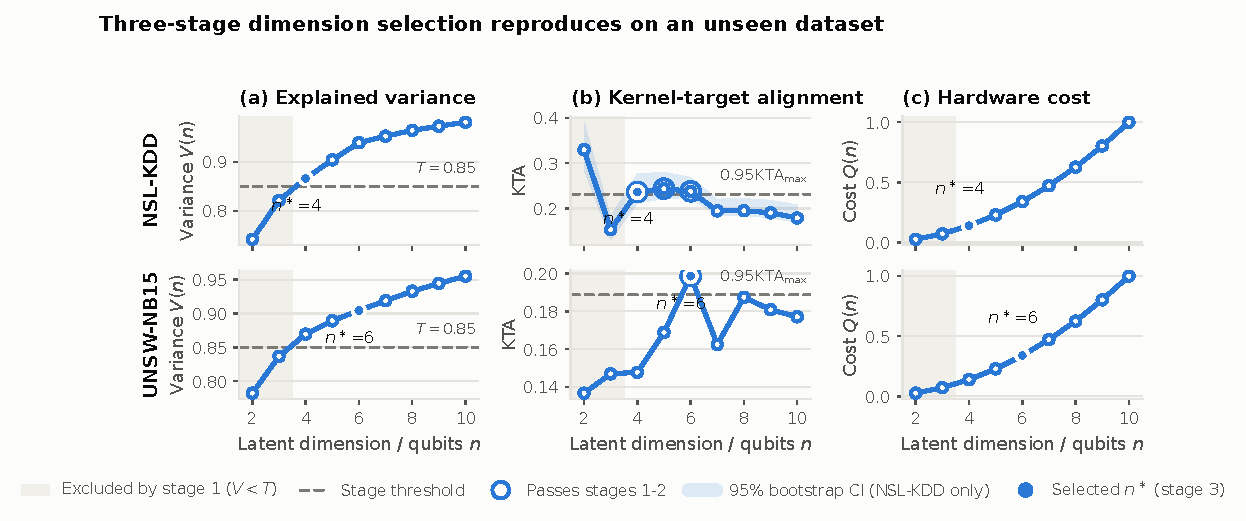
\includegraphics[width=\textwidth]{figs_revision/fig5_c1_dimension_selection.pdf}
  \caption{%
    \textbf{The three-stage dimension-selection rule, applied unchanged to two
    datasets.}
    Rows: NSL-KDD (top) and UNSW-NB15 (bottom). Columns: (a) explained variance
    $V(n)$, (b) kernel-target alignment, (c) CNOT-weighted hardware cost $Q(n)$.
    The rule is applied in a fixed order and has no tunable weights: stage~1
    discards every $n$ with $V(n)<T=0.85$ (shaded); stage~2 keeps those with
    $\mathrm{KTA}(n)\ge 0.95\,\mathrm{KTA}_{\max}$ among the survivors (open
    circles); stage~3 selects the cheapest survivor (filled marker).
    The same procedure, with no parameter changed, returns $n^\ast=4$ on
    NSL-KDD and $n^\ast=6$ on UNSW-NB15, and $n^\ast=6$ is recovered on
    $10/10$ independent UNSW subsets and under every threshold perturbation we
    tested. The selected dimension is therefore a \emph{property of the dataset
    produced by a transferable procedure}, not a constant carried over from one
    experiment. Bootstrap intervals ($B=200$) are available for NSL-KDD only.
    Note that stage~1 is what removes $n=2$ on NSL-KDD despite its high
    alignment: a kernel can be well aligned on a representation that has
    already discarded most of the signal.}
  \label{fig:c1-selection}
\end{figure*}

% ---------------------------------------------------------------------
% Hinh 9 -- learning curve + crossover, NSL-KDD
% ---------------------------------------------------------------------
\begin{figure*}[t]
  \centering
  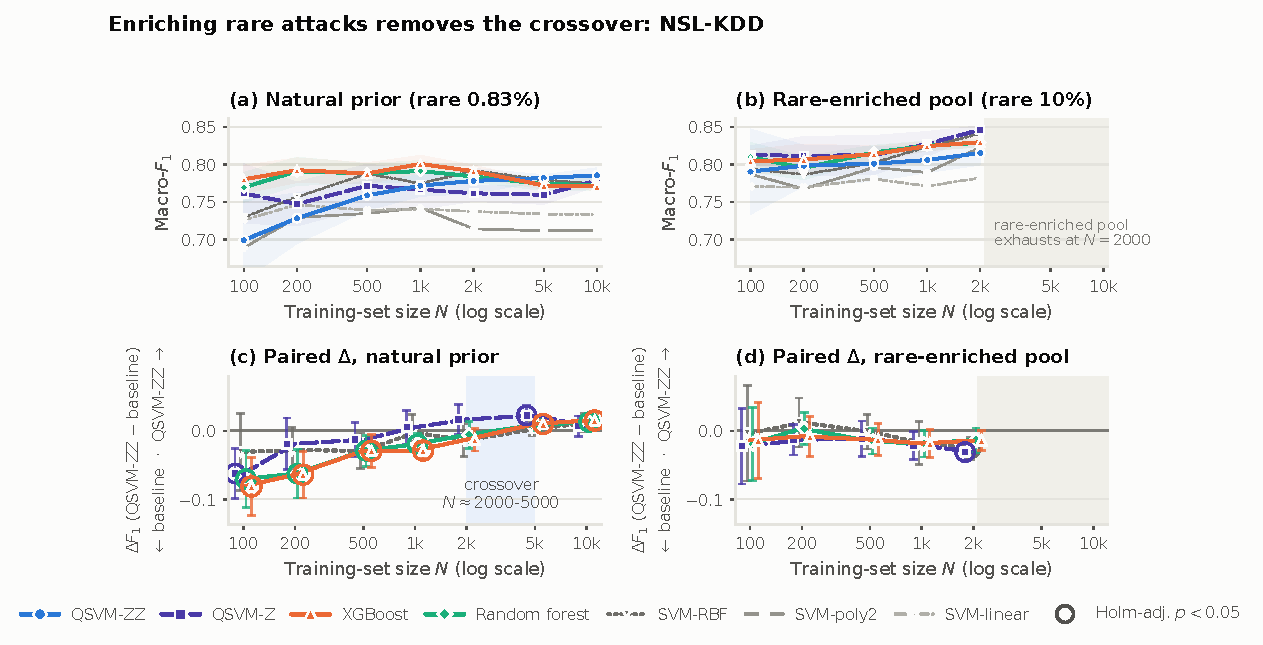
\includegraphics[width=\textwidth]{figs_revision/fig9_learning_curve_nslkdd.pdf}
  \caption{%
    \textbf{Rare-attack enrichment, not sample size alone, decides whether the
    quantum kernel leads on NSL-KDD.}
    (a,~b) Mean macro-$F_1$ over 10 runs on the full KDDTest+ set, with 95\%
    confidence bands on the highlighted series; (c,~d) the corresponding paired
    differences $\Delta F_1=$ QSVM-ZZ $-$ baseline with 95\% intervals, circled
    where the Holm-adjusted $p<0.05$ within the baseline family. All four panels
    share one $N$ axis so the two sampling regimes can be read against each
    other; the rare-enriched pool exhausts at $N=2000$ (shaded).
    Under the natural class prior (rare classes $0.83\%$) the ordering reverses
    between $N=2000$ and $N=5000$ (band in~c), and QSVM-ZZ leads XGBoost by
    $+0.015$ at $N=10^4$ (Holm $p=0.008$). Drawing the training sets from the
    rare-enriched pool used by the submitted version (rare $10\%$, a
    $12\times$ enrichment) removes the reversal entirely (d).
    The crossover is not an artefact of re-tuning: freezing the hyper-parameters
    at their fixed values reproduces it at the same location
    (Table~\ref{tab:crossover-arms}).
    SVM-RBF is retained throughout because it, not XGBoost, is the strongest
    classical baseline at $N=10^4$ ($0.774$ vs $0.771$); QSVM-ZZ never beats it
    significantly at any $N$ on this dataset.}
  \label{fig:learning-curve}
\end{figure*}

% ---------------------------------------------------------------------
% Hinh 10 -- ban do che do
% ---------------------------------------------------------------------
\begin{figure*}[t]
  \centering
  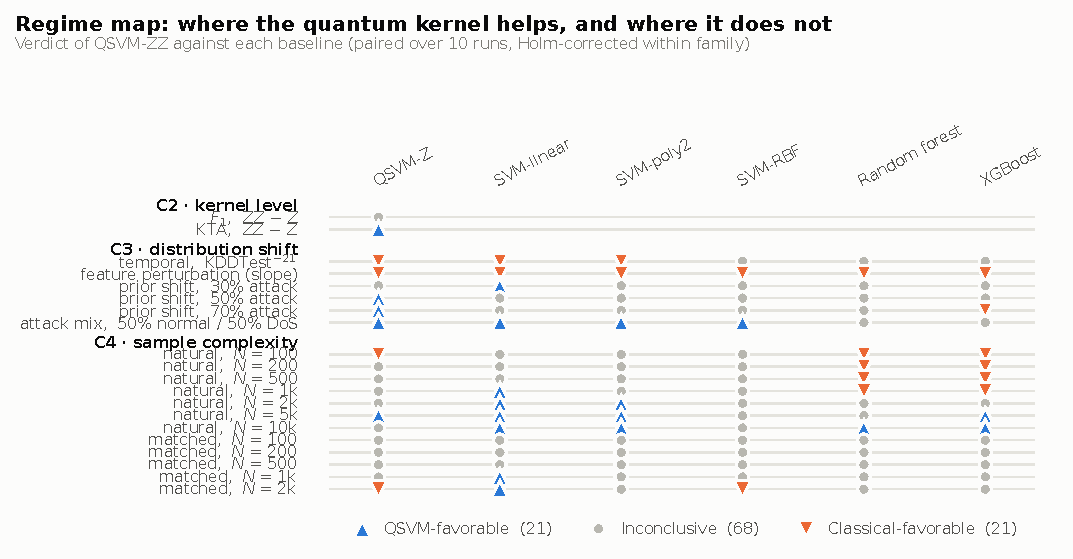
\includegraphics[width=\textwidth]{figs_revision/fig10_regime_map.pdf}
  \caption{%
    \textbf{Regime map: 110 controlled comparisons of QSVM-ZZ against six
    baselines.}
    Each cell is one paired comparison over 10 runs, Holm-corrected within its
    baseline family (\emph{entanglement}: QSVM-Z; \emph{classical kernel}:
    linear, poly2, RBF; \emph{strong tabular}: random forest, XGBoost).
    Verdicts are encoded by both colour and glyph so the figure survives
    greyscale printing.
    The distribution is the result: 21 QSVM-favourable, 21 classical-favourable
    and 68 inconclusive cells. We report this rather than a headline win because
    the honest summary of the evidence is that the quantum kernel helps in
    identifiable regimes---low label prior, shifted attack composition, larger
    training sets---and does not help, or loses, elsewhere. A single aggregate
    number over this table would hide exactly the structure the paper is about.}
  \label{fig:regime-map}
\end{figure*}

% ---------------------------------------------------------------------
% Hinh 11 -- chuyen giao UNSW-NB15
% ---------------------------------------------------------------------
\begin{figure*}[t]
  \centering
  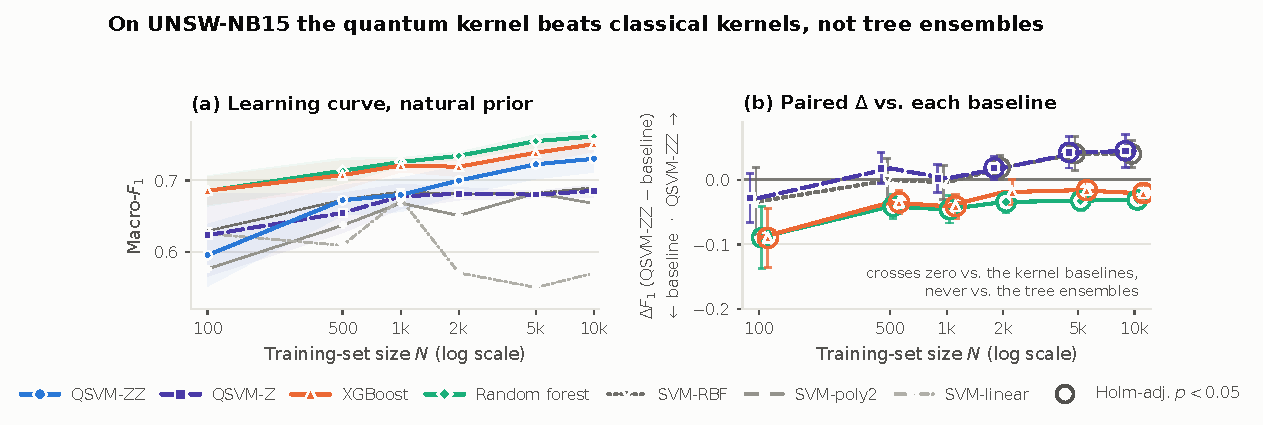
\includegraphics[width=\textwidth]{figs_revision/fig11_unsw_transfer.pdf}
  \caption{%
    \textbf{What transfers to UNSW-NB15, and what does not.}
    (a) Mean macro-$F_1$ over 10 runs on the official UNSW-NB15 test set;
    (b) paired $\Delta F_1$ against each baseline, circled where the
    Holm-adjusted $p<0.05$.
    The dimension-selection rule transfers (Fig.~\ref{fig:c1-selection}) and so
    does the entanglement ablation, which is roughly twice as large here
    ($+0.045$, Holm $p=0.002$ at $N=10^4$) as the largest significant effect we
    measure on NSL-KDD ($+0.022$ at $N=5000$), and which holds at every
    $N\ge 2000$ rather than at a single point. The sample-complexity crossover
    does \emph{not} transfer: against both tree ensembles the difference keeps its sign at
    every $N$ we tested. Against the kernel baselines it does change sign, and
    QSVM-ZZ leads SVM-RBF from $N\ge 2000$ ($+0.040$, Holm $p=0.006$ at
    $N=10^4$)---the opposite of NSL-KDD, where that comparison is never
    significant. The rare-class advantage does not transfer either, because the
    UNSW rare classes are simply easier (recall $0.95$--$0.99$ for all
    seven models).
    A single dataset would have supported a broader claim than the evidence
    warrants.}
  \label{fig:unsw-transfer}
\end{figure*}
